\documentclass[../../main.tex]{subfiles}

\graphicspath{{images/Maschinentechnik/}{../../images/Maschinentechnik/}}

\lstset{basicstyle=\small,
      showstringspaces=false,
      commentstyle=\color{black},
      keywordstyle=\color{blue}
    }

\begin{document}

%Vergleich zwischen Konzeptlösung und Funktionsmuster (Bewertung der Lösung) 
Das Konzept aus PREN1 konnte in den meisten Punkten im PREN2 so wie geplant umgesetzt werden. Nötige Änderungen sind in diesem Kapitle beschrieben und begründet. Einige Sachen mussten angepasst werden, andere wurden aus Zeitgründen weggelassen. Die weggelassenen Teilkonzepte sind allerdings alle nicht zwingend notwendig um die Aufgebenstellung zu erfüllen.\\

\subsection{Elektronik}
In diesem Kapitel wird das Konzept für die Elektronik bewertet und allfällige Änderungen beschrieben.

\subsubsection{Bewertung}
Ausser den Änderungen, welche in Kapitel \ref{bewertung_et_aenderungen} beschrieben sind konnte das Konzept wie geplant umgesetzt werden. Die Teilkonzepte für die Aktoren und Sensoren konnten erfolgreich umgesetzt werden.

\subsubsection{Änderungen} \label{bewertung_et_aenderungen}
Weggelassen wurden die Strommessung und der Parksensor. Eine weitere Anpassung ist das Prinzip wie der Quadraturencoder für den Antrieb ausgewertet wird und daraus die Geschwindigkeit bestimmt wird. Auch wurde eine Änderung für den Quadraturencoder für den Schwenker durchgeführt, damit auch erkann wird wenn sich der Schwenker rückwärts dreht.\\
Im Folgenden sind die Gründe dafür erläutert.\\

\textbf{Strommessung}\\
Die Strommessung ist auf der ersten Version des PCB nicht möglich, da ein Fehler bei der Pinbelegung des Operationsverstärkers ist. Dieser Fehler konnte aus Zeitgründen nicht mehr korrigiert werden und da die Information zum Strom nicht nötig ist um die Aufgabe zu erfüllen fiel der Entscheid dieses Teilkonzept ganz zu verwerfen.\\

\textbf{Parksensor}\\
Die Distanz zum Haltesignal kann direkt über die Auswertung der Kamera bestimmt werden. Dies reduziert den Hardwareaufwand für die Elektronik und Mechanik.\\

\textbf{Quadraturencoder Antrieb}\\
Das im PREN1 angedachte Konzept basierte darauf die Zeit zwischen zwei Impulsen zu messen und daraus die Geschwindigkeit zu bestimmen. Dies stellte sich in der Umsetzung jedoch als zu wenig zuverlässig heraus. Vorallem im Zusammenhang mit der Regelung (beschrieben in Kapitle \ref{et_sw_modul_drive}) wurde es mit der unzuverlässigen Auswertung des Encoders unmöglich eine konstante Geschwindigkeit zu halten. Daher wurde das Prinzip angepasst, dass die Impulse des Encoders über eine bestimmte Zeit gezählt werden und daraus die Geschwindigkeit bestimmt wird (siehe Kapitle \ref{et_sw_modul_drive}).\\

\textbf{Quadraturencoder Schwenker}\\
In den ersten Tests kam es vor, dass der Schwenker während des Einfahren wieder ein wenig rückwärts rutschte. Mit dem Angedachten Prinzip zum Zählen der Impulse an einem Kanal kann aber die Richtung nicht festgestellt werden und ein Impuls rückwärts wird gleich interpretiert wie ein Impuls vorwärts. Dies verfälscht die Bestimmung der Position und macht es unmöglich sicherzustellen, dass der Schwenker die richtige Position erreicht. Um zu erkennen in welche Richtung sich der Schwenker dreht wurde der zweite Kanal des Quadraturencoders auf einen Pin vom Mikrocontroller verbunden. Durch das Auslesen dieses Pins bei einer positiven Flanke am anderen Kanal kann die Drehrichtung bestimmt werden. (siehe Abbildung \ref{fig:et_encoder} auf Seite \pageref{fig:et_encoder}) Mit dieser Information kann also sichergestellt werden, dass der Schwenker weit genug dreht.\\ 

\subsection{Informatik}

\textbf{Tafel- \& Nummererkennung}\\
Das im PREN 1 erstellte Konzept im Bereich der Tafel- \& Nummererkennung musste während PREN 2 im Bereich der Hardware sowie im Bereich der Software Anpassungen vorgenommen werden. Wie im Kapitel \ref{numberdetection} beschrieben, musste im Bereich der Hardware auf einen rechenstärkeren Raspberry PI 3 A+ gewechselt werden. Dank der Budgetreserve und der minimalen Hardwareanpassung konnte dies ohne Probleme vorgenommen werden. Im Bereich der Software wurde bei der Nummererkennung auf die Software Teseract OCR gewechselt. Dies aus den Gründen der Einfachheit und der Effizienz. 

\textbf{Akustik}\\
Der Buzzer wurde bereits in Pren1 getestet, dementsprechend ist das Ergebnis gemäss den Erwartungen. Mit der kompakten Struktur und dem geringen Stromverbrauch ist er eine ideale Komponente für Projekte dieser Grössenordnung.

\textbf{Beschleunigungssensor}\\
Die Messung der Beschleunigung erfolgt wie erwartet. Bei der Umrechnung herschen noch kleinere Unsicherheiten bezüglich der Genauigkeit. Der Beschleunigungssensor findet leider keine Anwendung im endgültigen Produkt, weil wir bereits die Geschwindigkeitsdaten des Motors auswerten.

\textbf{WebApp}\\
Die WebApp wurde in PREN2 entworfen und entwickelt, somit gibt es keine Erwartungen an diese Komponente. Das Endergebnis entspricht ziemlich genau unseren Vorstellungen.

\textbf{Würfelaufnahme}\\
Das Grundkonzept wurde in PREN1 definiert und umgesetzt. Für das endgültige Produkt wurden kleine Änderungen vorgenommen. Der Verlauf der Kurvenscheibe wurde angepasst und die Führung des Würfels optimiert. Nun kann der Aufbau den Anforderungen gerecht werden. 

\pagebreak

\subsection{Maschinentechnik}

\textbf{Teststrecke}\\
Die grösste Herausforderung an das Fahrwerk besteht bei einer Doppelkurve mit engem Radius (siehe oben mitte in Abbildung \ref{fig:teststrecke1}). Ansonsten erfüllt die Lokomotive die Anforderungen an die Strecke. Sie berührt das Lichtraumprofil und kein anderes Element auf der Testrecke, mit einer Ausnahme, dem Holzwürfel. Ein Problem für die Mechanik stellt die enge Doppelkurve dar, da dadurch grosse Kräfte an der Lokomotive entstehen, welche aber durch die Kurvenführung weitgehen behoben wird.\\

\begin{figure}[H]
    \centering
    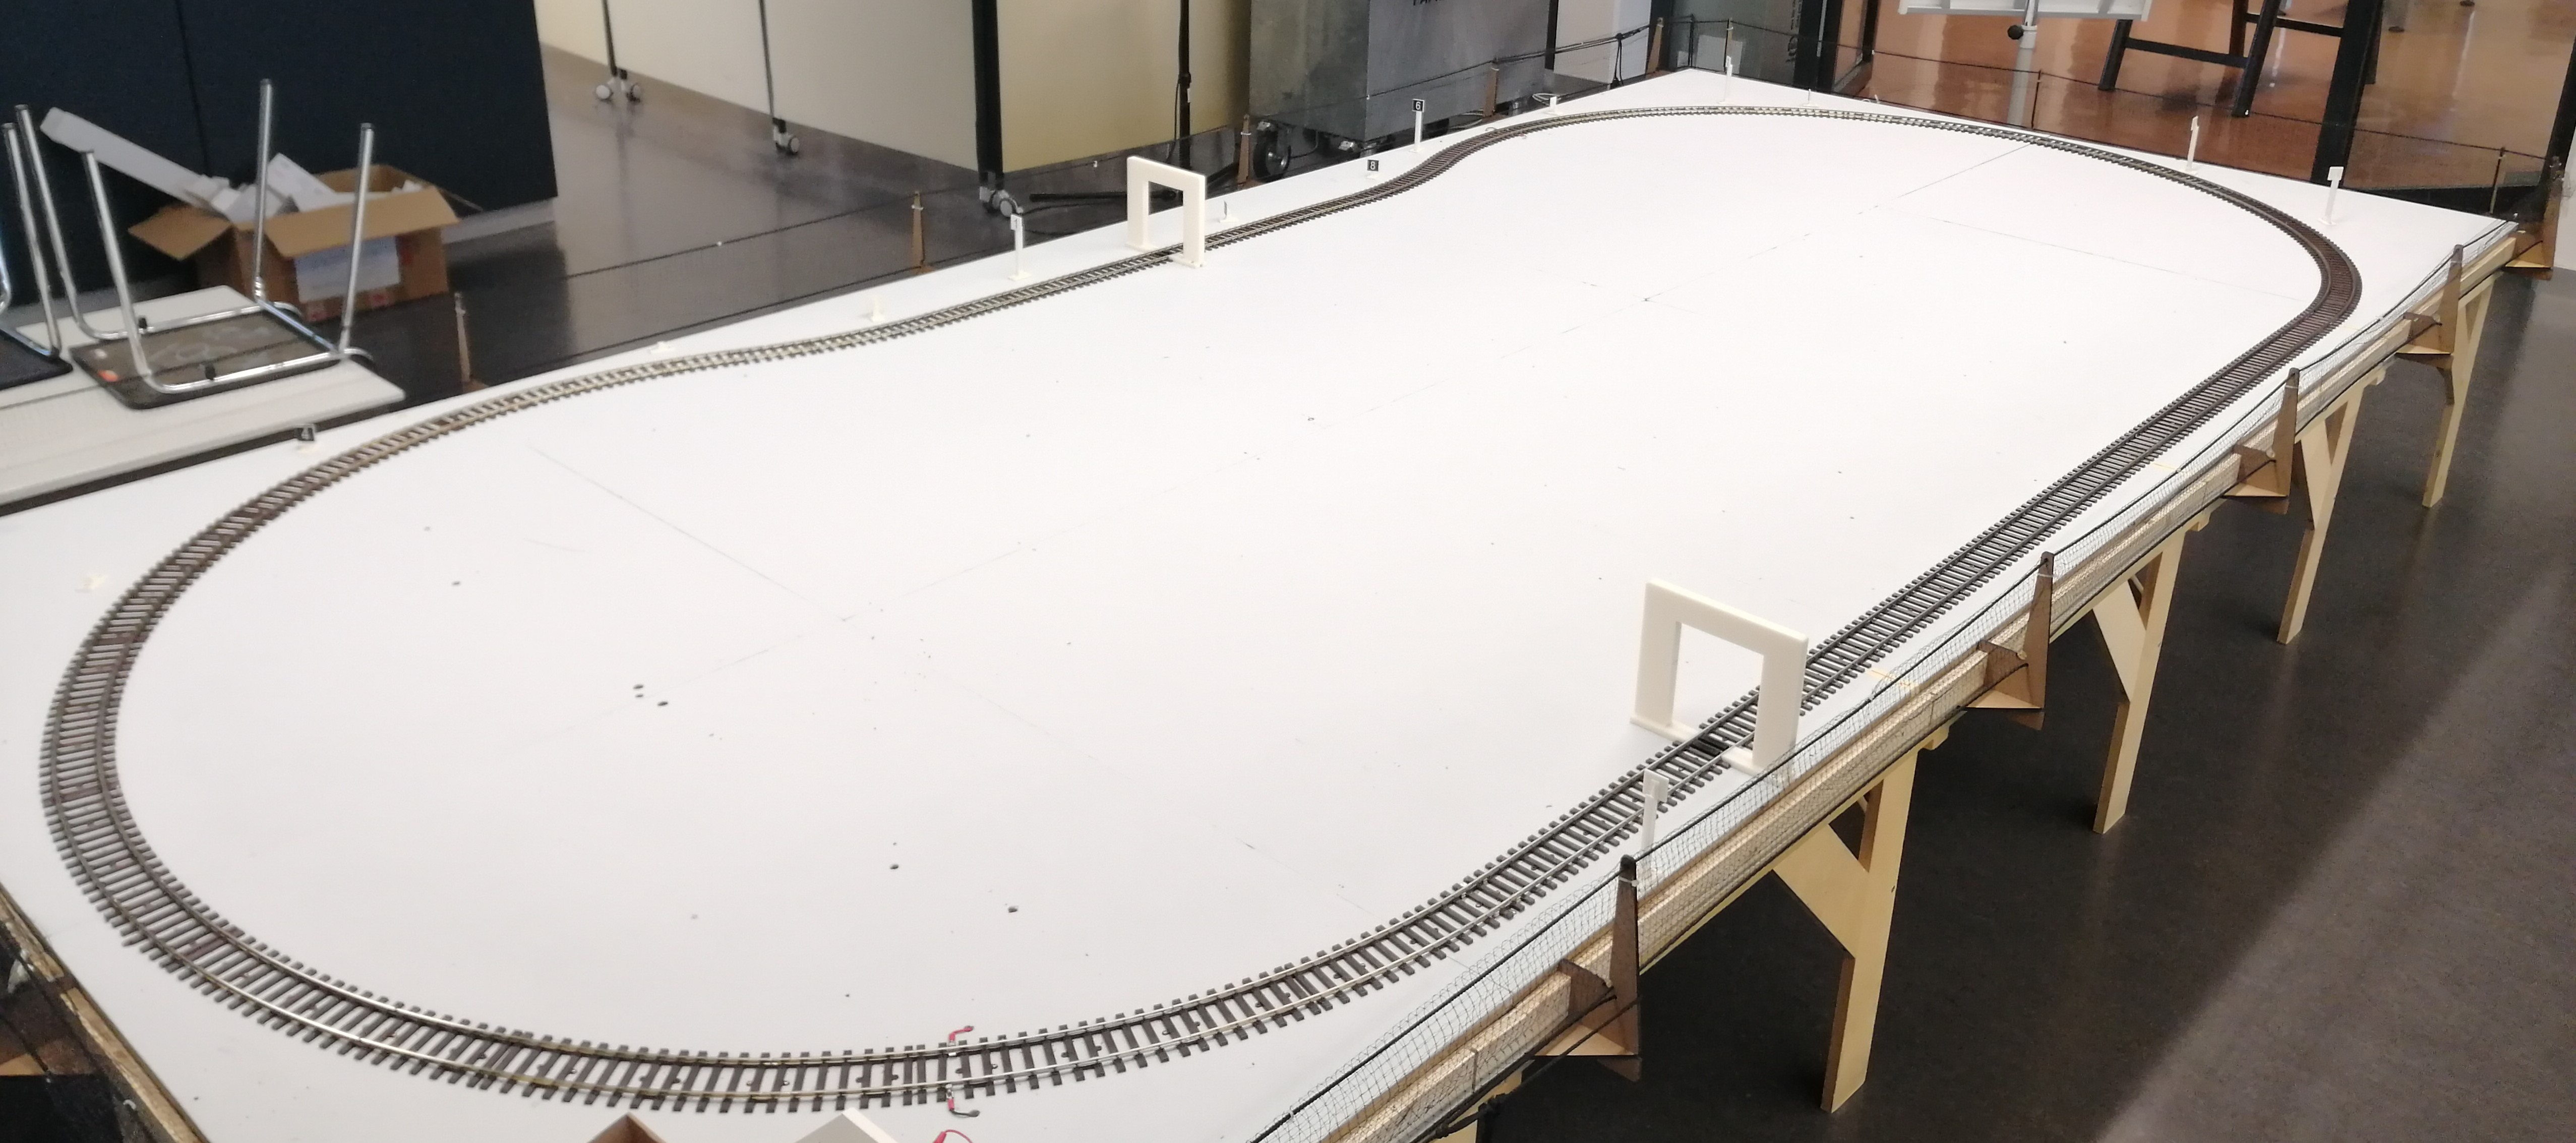
\includegraphics[width=0.8\textwidth]{teststrecke1.PNG}
    \caption {Aufbau Teststrecke}
    \label{fig:teststrecke1}
  \end{figure}

\textbf{Antriebswagen}\\
Der Antriebswagen (siehe Abbildung \ref{fig:antriebswagen3}) wie auch der Führungswagen sind im allgmeinen wie konzipiert und konsturiert realisiert. In der Umsetzung wurden beim Antriebswagen zusätzlich zwei weitere Schleifkontakte für die bessere Gewährleistung der Stromabnahme und ein Vorrichtung für die Kurvenführung angebracht. Die Grösse und Form der Räder (siehe Abbildung \ref{fig:raeder}) wurde etwas angepasst, da die Gefahr bestand, dass die Lokomotive an den Gleisen hängen bleibt. Die genauen Änderungen der Räder werden im nächsten Absatz ausführlicher vorgestellt.\\

\begin{figure}[H]
  \centering
  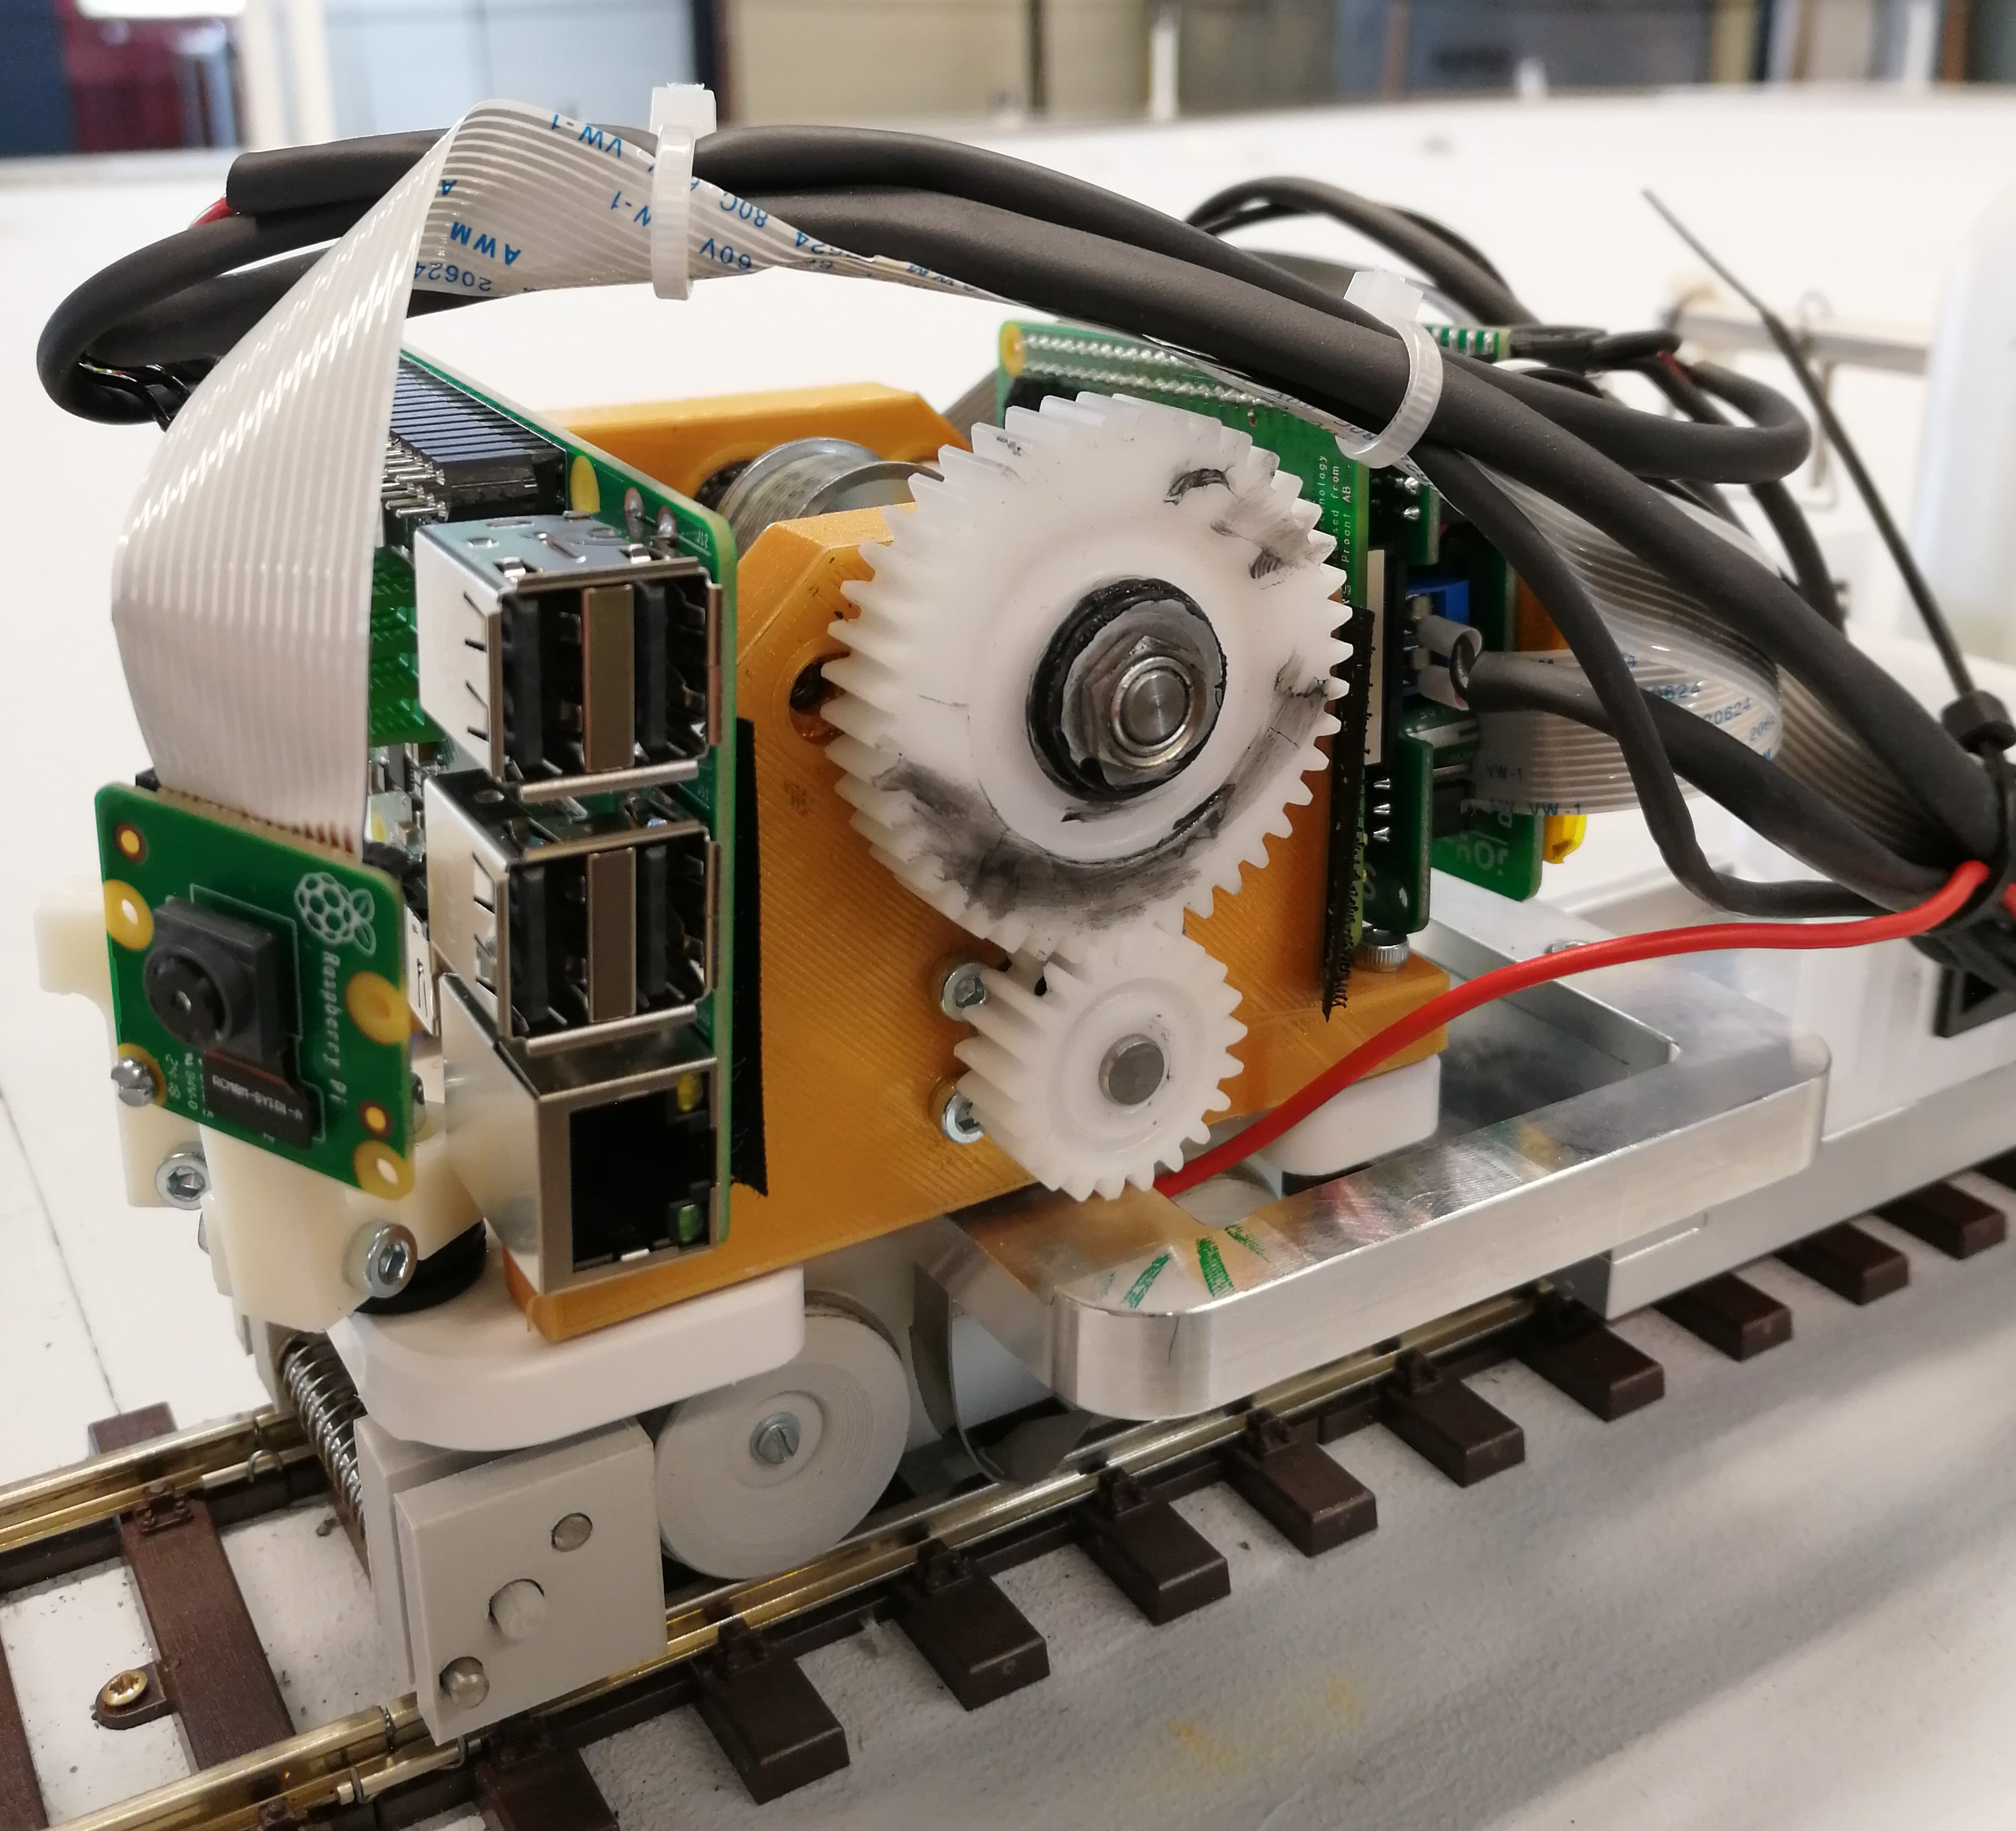
\includegraphics[width=0.48\textwidth]{antriebswagen1.PNG}
  \caption {Antriebswagen}
  \label{fig:antriebswagen3}
\end{figure}

\pagebreak

\textbf{Beschleunigung und Geschwindigkeit}\\
Bei den Probefahrten auf der vorgebenen Teststrecke (siehe Abschnitt "Teststrecke") hat sich eine maximale Beschleunigung von 1 Meter pro Sekunde im Quadrat herausgestellt. Diese ergibt sich durch das Moment welches über das Getriebe auf die Räder übertragen wird, die Normalkraft des Zuges und der Reibwert zwischen Räder und Gleis. Dieser Wert entstand durch Messungen mit einem Beschleunigungsensor. Der berechnete Wert lag 2.94 Meter pro Sekunde im Quadrat. Die Differenz lässt sich durch den abweichenden Reibwert und die Masse erklären.\\
Gemäss den Messungen auf der Teststrecke ist eine maximale Geschwindigkeit von 2.2 Meter pro Sekunde erreichbar. Der limitierende Faktor ist nicht das Kippen beziehungseise entgleisen in der Kurve, sondern der Motor. Der Motor erreicht dieser Geschwindigkeit seine maximale Leistung mit den gegebenn Werten des Stromes und der Spannung. Somit fährt die Lokomotive 1.7 Meter pro Sekunde schneller als im Anforderungskatalog deklariert wurde und etwa 0.7 Meter pro Sekunde schneller als der theoretisch berechnete Wert. An Hand dieser Ergebnisse ist ersichtlich, dass der Schwerpunkt optimaler liegt, als angenommen wurde und zusätzlich die Kurvenvorrichtung dazu beiträgt, dass die Lokomotive in der Kurve schneller fahren kann.\\

\textbf{Wagenräder}\\
Die Räder der Lokomotive sind für zwei Bereiche vorgesehen. Einerseits gibt es Räder für den Antriebswagen und andererseits solche für den Führungswagen. Die Räder für den Fürhungswagen haben im Gegensatz zu denen des Antriebswagens keine spezielle Bearbetiung. In einem ersten Veruch wurden die Reifen mit einem O-Ring versehen. Da der Anpressdruck durch das Gewicht der Lokomotive zu gering war und die Fuge nicht gleichmässig mit der Gummimasse gefüllt wurde, kippte der Zug leicht auf den Gleisen hin und her, da zusätzlich der Absatz für die Führung zu kurz war. In einem nächsten Schritt wurde ein Gummispray Schicht für Schicht auf die Räder gesprayt. Jedoch weissten diese bei der Testfahrt bereits grossen Verschleiss auf und ist somit für die Forderung nicht ausreichend. Als letzter und funktionsfähiger Versuch wurden die Räder mit einem speziellen Gummiband umwickelt. Die Funktion ist erfüllt und der Verschleiss hält sich in einem vernünftigen Rahmen. Bei den Antriebsrädern wie auch bei den Führungsrädern ist der Durchmesser etwas grösser und die Kontur leicht angepasst.\\

\begin{figure}[H]
  \centering
  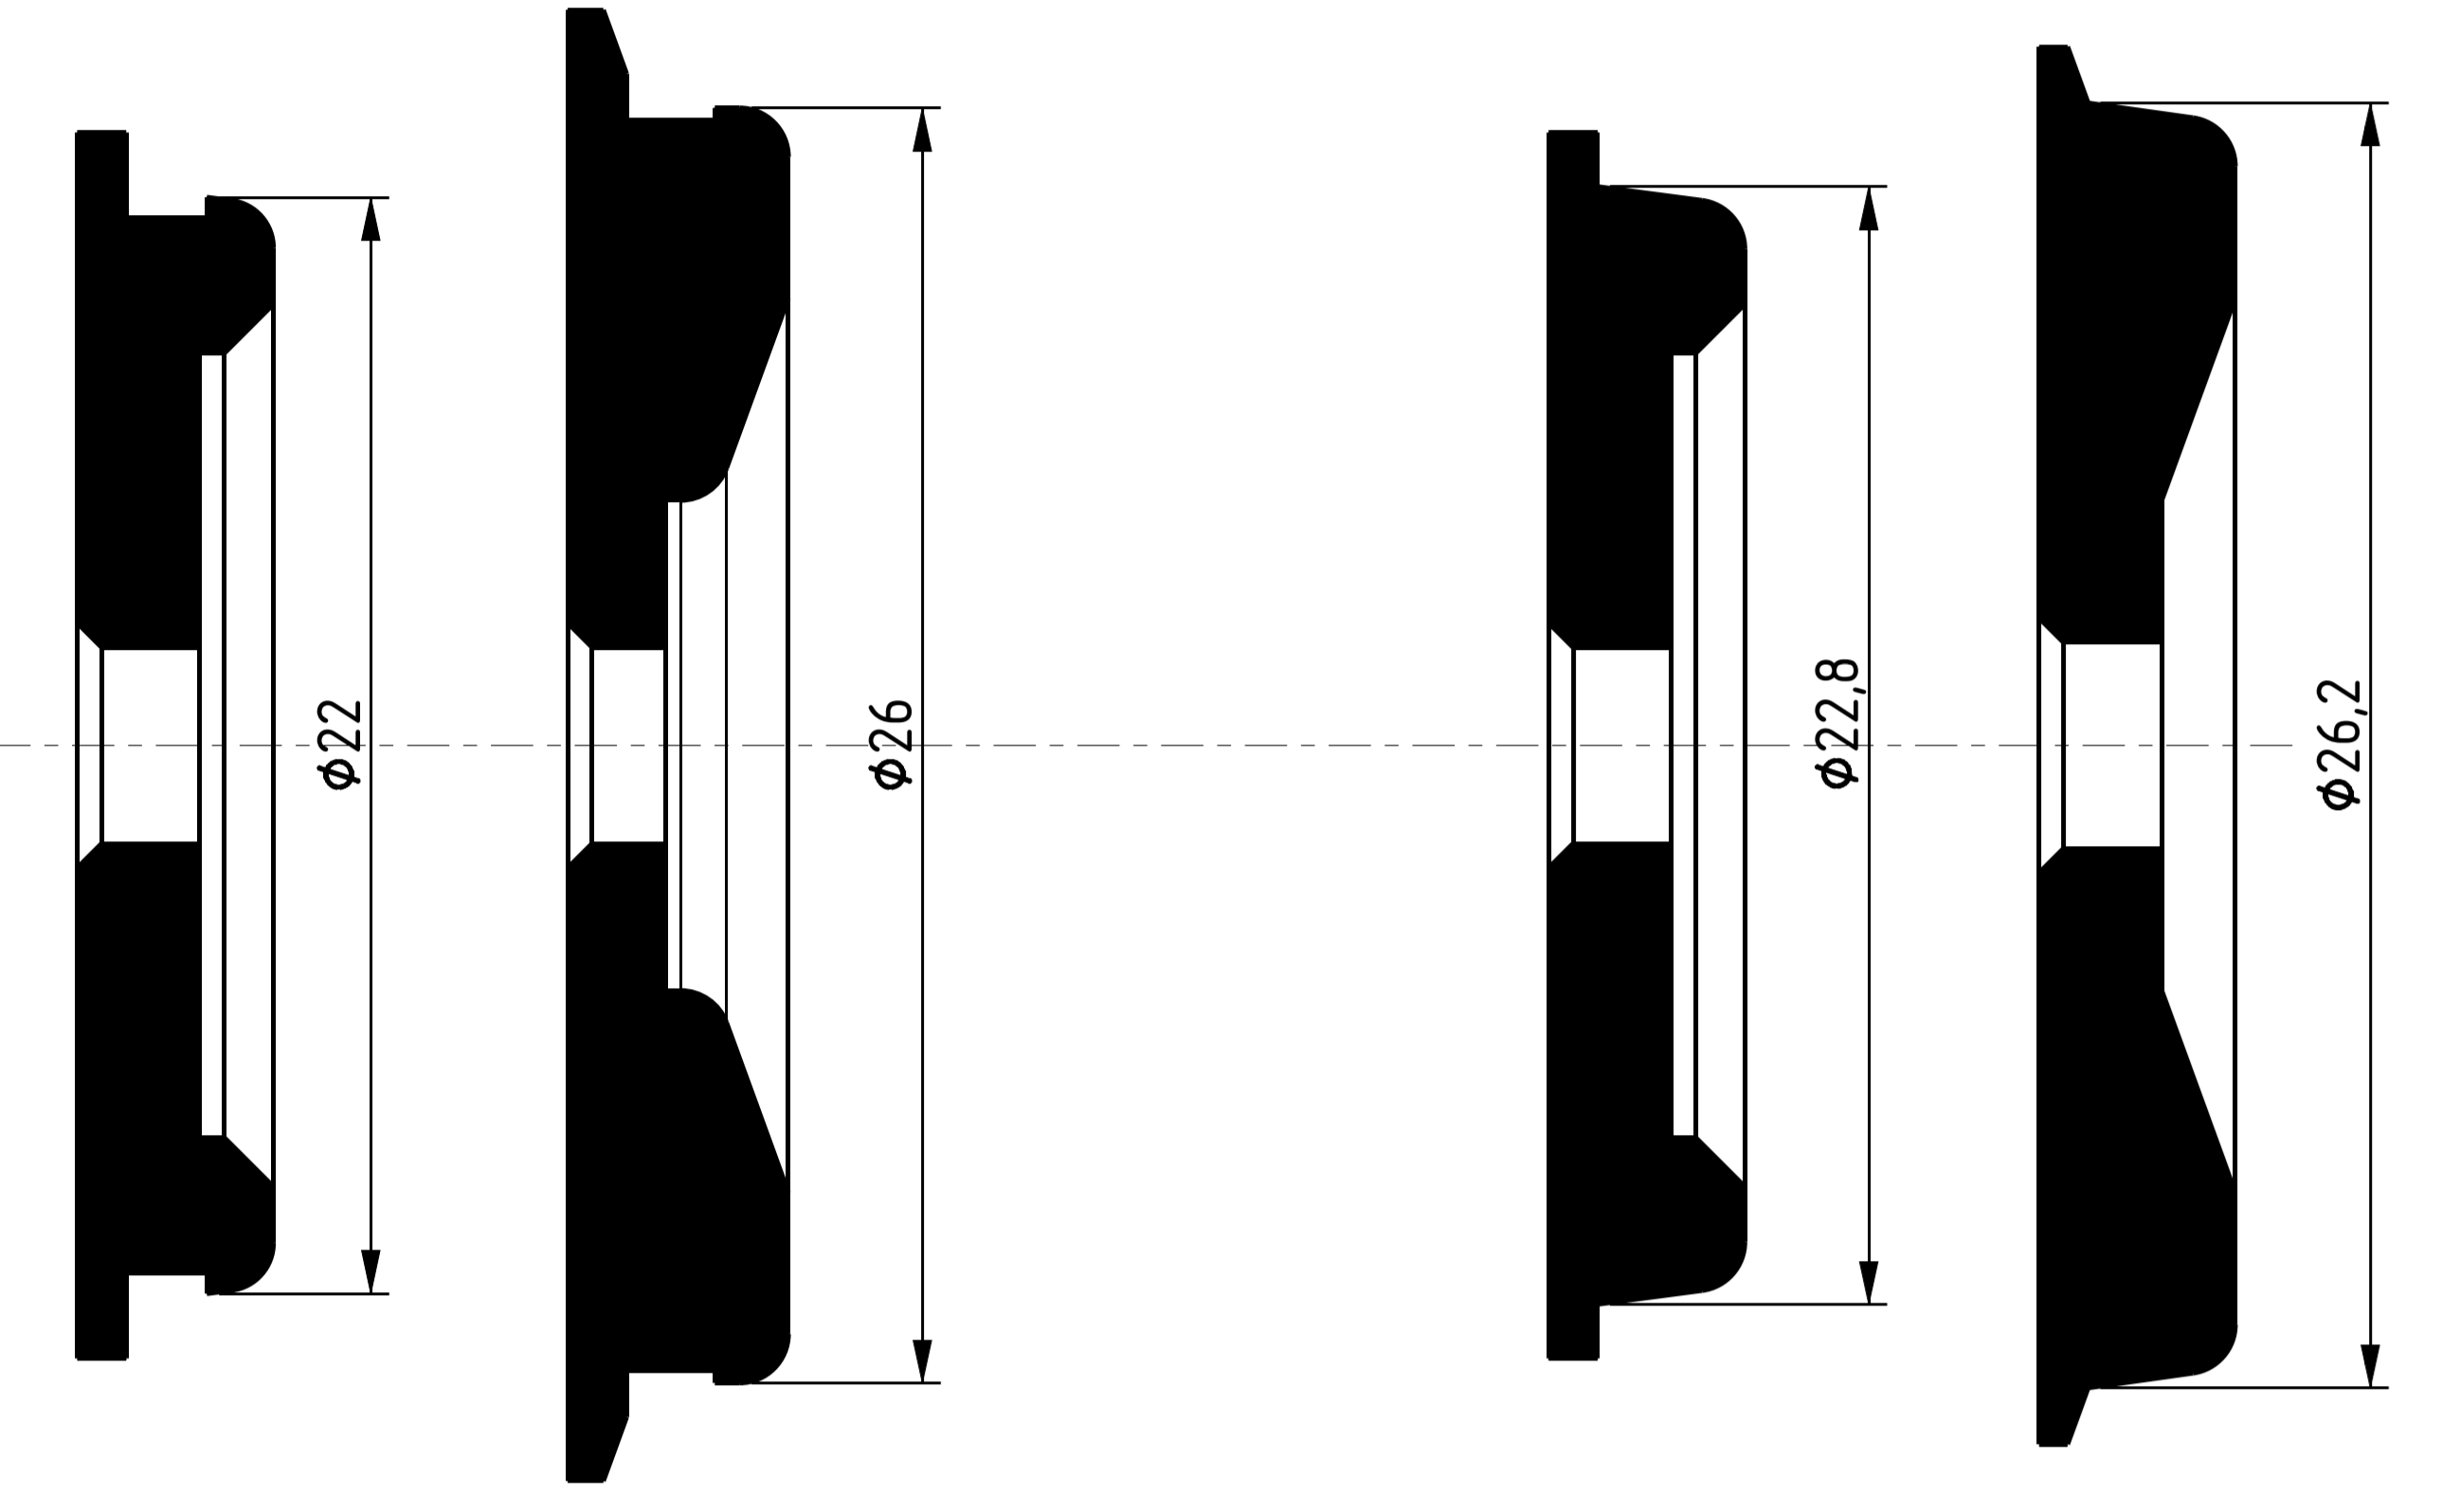
\includegraphics[width=0.6\textwidth]{wagenraeder.PNG}
  \caption {Räder Antriebswagen bzw. Führungswagen - Alt vs. Neu}
  \label{fig:raeder}
\end{figure}

\pagebreak

\textbf{Stromabnahme}\\
In einem ersten Versuch wurde die Stromabnahme nur an einem Ort, dem Führungswagen, abgenommen. Jedoch ist die Gefahr gross, dass die Schleifkontakte bereits bei kleinsten Unebenheiten der Strecke den Kontakt verlieren und das System zum Absturz bringen. Somit wurden zusätzlich zwei Schleifkontakte am Antriebswagen befestigt, welche die Gefahr minimiert. Die Stromabnahme funktioniert nun mit der gewünschten Zuverlässigkeit.

\textbf{Kurvenführung}\\
Die Kurvenführung wurde in mehreren Testfahrten getestet und zeigte die gewünschten Effekte auf. Lediglich die Feder beziehungsweise die Federrate musste angepasst werden, damit der Anpressdruck der Stahlstifte genügend hoch ist und so der Zentripedalkraft der Lokomotive entgegenwirken kann.

\end{document}